\documentclass[10pt,a4paper]{article}
\usepackage[right=0.5cm, left=0.5cm,top=1cm,bottom=1.5cm]{geometry}
\usepackage{enumitem}
\usepackage{graphicx}
\usepackage{array, tasks}
\usepackage{blindtext}
\usepackage{fontspec}
\usepackage{amsmath,amsfonts,amssymb,mathrsfs,amsthm}
\usepackage{fancyhdr}
\usepackage{xcolor}
\usepackage{booktabs}
\usepackage[font={bf}]{caption}
% \captionsetup[table]{box=colorbox,boxcolor=orange!20}
\usepackage{float}
\usepackage{esvect}
\usepackage{tabularx}
\usepackage{pifont}
\usepackage{colortbl}
 \usepackage{fancybox}
 \mathversion{bold}
 \usepackage{pgfplots}
 % \usepackage[utf8]{inputenc}
\usepackage{tikz}
 \usepackage[tikz]{bclogo}%
 \usepackage{mathpazo}
\usepackage{ulem}
\usepackage{yagusylo}
\usepackage{textcomp}
\usepackage{blindtext}
\usepackage{multicol}
\usepackage{varwidth}
\usetikzlibrary{calc,intersections}
\usepackage{pgfplots}
%\usepackage{fourier}
\pgfplotsset{compat=1.11}
\usepackage{tkz-tab}
\usepackage{xcolor}
\usepackage{color}
\usetikzlibrary{calc}
\mathchardef\times="2202
\usepackage[most]{tcolorbox}
\definecolor{lightgray}{gray}{0.9}
\definecolor{ocre}{RGB}{0,244,244} 
\definecolor{head}{RGB}{255,211,204}
\definecolor{browndark}{RGB}{105,79,56}
%\RequirePackage[framemethod=default]{mdframed}
\usepackage{tikz}
\usetikzlibrary{calc,patterns,decorations.pathmorphing,arrows.meta,decorations.markings}
\usetikzlibrary{arrows.meta}
\makeatletter
\tcbuselibrary{skins,breakable,xparse}
\tcbset{%
  save height/.code={%
    \tcbset{breakable}%
    \providecommand{#1}{2cm}%
    \def\tcb@split@start{%
      \tcb@breakat@init%
      \tcb@comp@h@page%
      \def\tcb@ch{%
        \tcbset{height=\tcb@h@page}%
        \tcbdimto#1{#1+\tcb@h@page-\tcb@natheight}%
        \immediate\write\@auxout{\string\gdef\string#1{#1}}%
        \tcb@ch%
      }%
      \tcb@drawcolorbox@standalone%
    }%
  }%
}
\newcommand{\Lim}{\displaystyle\lim}
\makeatother
\newcommand{\oij}{$\left( \text{O};\vv{i},\vv{j} , \vv{k}\right)$}
\colorlet{darkred}{red!30!black}
\newcommand{\red}[1]{\textcolor{darkred}{ #1}}
\newcommand{\rr}{\mathbb{R}}
\renewcommand{\baselinestretch}{1.2}
 \setlength{\arrayrulewidth}{1.25pt}
\usepackage{titlesec}
\usepackage{titletoc}
\usepackage{minitoc}
\usepackage{ulem}
%--------------------------------------------------------------

\usetikzlibrary{decorations.pathmorphing}
\tcbuselibrary{skins}

%%%%%%%%%%%
%-------------------------------------------------------------------------
\tcbset{
        enhanced,
        colback=white,
        boxrule=0.1pt,
        colframe=brown!10,
        fonttitle=\bfseries
       }
\definecolor{problemblue}{RGB}{100,134,158}
\definecolor{idiomsgreen}{RGB}{0,162,0}
\definecolor{exercisebgblue}{RGB}{192,232,252}
\definecolor{darkbrown}{rgb}{0.4, 0.26, 0.13}

\newcommand*{\arraycolor}[1]{\protect\leavevmode\color{#1}}
\newcolumntype{A}{>{\columncolor{blue!50!white}}c}
\newcolumntype{B}{>{\columncolor{LightGoldenrod}}c}
\newcolumntype{C}{>{\columncolor{FireBrick!50}}c}
\newcolumntype{D}{>{\columncolor{Gray!42}}c}

\newcounter{mysection}
\newcounter{mysubsection}
\newcommand{\mysection}[1]{%
    \stepcounter{mysection} % Increment the counter
    \textcolor{red}{\LARGE\themysection. #1 :}
}
\newcommand{\mysubsection}[2]{
    \stepcounter{mysubsection}
    \textcolor{red}{\large \themysection.#1. #2 :}
}
% \textcolor{red}{\LARGE\bfseries 1. Les équation du deuxiéme degrée :}

%------------------------------------------------------
\newtcolorbox[auto counter]{Définition}{enhanced,
before skip=2mm,after skip=2mm,
colback=yellow!20!white,colframe=lime,boxrule=0.2mm,
attach boxed title to top left =
    {xshift=0.6cm,yshift*=1mm-\tcboxedtitleheight},
    varwidth boxed title*=-3cm,
    boxed title style={frame code={
                        \path[fill=lime]
                            ([yshift=-1mm,xshift=-1mm]frame.north west)  
                            arc[start angle=0,end angle=180,radius=1mm]
                            ([yshift=-1mm,xshift=1mm]frame.north east)
                            arc[start angle=180,end angle=0,radius=1mm];
                        \path[left color=lime,right color = lime,
                            middle color = lime]
                            ([xshift=-2mm]frame.north west) -- ([xshift=2mm]frame.north east)
                            [rounded corners=1mm]-- ([xshift=1mm,yshift=-1mm]frame.north east) 
                            -- (frame.south east) -- (frame.south west)
                            -- ([xshift=-1mm,yshift=-1mm]frame.north west)
                            [sharp corners]-- cycle;
                            },interior engine=empty,
                    },
fonttitle=\bfseries\sffamily,
title={Définition ~\thetcbcounter}}
%------------------------------------------------------
\newtcolorbox[auto counter]{Proposition}{enhanced,
before skip=2mm,after skip=2mm,
colback=yellow!20!white,colframe=blue,boxrule=0.2mm,
attach boxed title to top left =
    {xshift=0.6cm,yshift*=1mm-\tcboxedtitleheight},
    varwidth boxed title*=-3cm,
    boxed title style={frame code={
                        \path[fill=blue]
                            ([yshift=-1mm,xshift=-1mm]frame.north west)  
                            arc[start angle=0,end angle=180,radius=1mm]
                            ([yshift=-1mm,xshift=1mm]frame.north east)
                            arc[start angle=180,end angle=0,radius=1mm];
                        \path[left color=blue,right color = blue,
                            middle color = blue]
                            ([xshift=-2mm]frame.north west) -- ([xshift=2mm]frame.north east)
                            [rounded corners=1mm]-- ([xshift=1mm,yshift=-1mm]frame.north east) 
                            -- (frame.south east) -- (frame.south west)
                            -- ([xshift=-1mm,yshift=-1mm]frame.north west)
                            [sharp corners]-- cycle;
                            },interior engine=empty,
                    },
fonttitle=\bfseries\sffamily,
title={Proposition ~\thetcbcounter}}
%------------------------------------------------------
\newtcolorbox[auto counter]{Théorème}{enhanced,
before skip=2mm,after skip=2mm,
colback=yellow!20!white,colframe=red,boxrule=0.2mm,
attach boxed title to top left =
    {xshift=0.6cm,yshift*=1mm-\tcboxedtitleheight},
    varwidth boxed title*=-3cm,
    boxed title style={frame code={
                        \path[fill=red]
                            ([yshift=-1mm,xshift=-1mm]frame.north west)  
                            arc[start angle=0,end angle=180,radius=1mm]
                            ([yshift=-1mm,xshift=1mm]frame.north east)
                            arc[start angle=180,end angle=0,radius=1mm];
                        \path[left color=red,right color = red,
                            middle color = red]
                            ([xshift=-2mm]frame.north west) -- ([xshift=2mm]frame.north east)
                            [rounded corners=1mm]-- ([xshift=1mm,yshift=-1mm]frame.north east) 
                            -- (frame.south east) -- (frame.south west)
                            -- ([xshift=-1mm,yshift=-1mm]frame.north west)
                            [sharp corners]-- cycle;
                            },interior engine=empty,
                    },
fonttitle=\bfseries\sffamily,
title={Théorème ~\thetcbcounter}}
%------------------------------------------------------
\newtcolorbox[auto counter]{Exemple}{
  % breakable,
  enhanced,
  colback=white,
  boxrule=0pt,
  arc=0pt,
  outer arc=0pt,
  title=Exemple ~\thetcbcounter,
  fonttitle=\bfseries\sffamily\large\strut,
  coltitle=problemblue,
  colbacktitle=problemblue,
  title style={
left color=exercisebgblue,
    right color=white,
    middle color=exercisebgblue  
  },
  overlay={
    \draw[line width=1pt,problemblue] (frame.south west) -- (frame.south east);
    \draw[line width=1pt,problemblue] (frame.north west) -- (frame.north east);
    \draw[line width=1pt,problemblue] (frame.south west) -- (frame.north west);
    \draw[line width=1pt,problemblue] (frame.south east) -- (frame.north east);
  }
}
%----------------------------------------------------
\newtcolorbox[auto counter]{Activité}{
  % breakable,
  enhanced,
  colback=white,
  boxrule=0pt,
  arc=0pt,
  outer arc=0pt,
  title=Activité ~\thetcbcounter,
  fonttitle=\bfseries\sffamily\large\strut,
  coltitle=problemblue,
  colbacktitle=problemblue,
  title style={
left color=yellow!50!white,
    right color=white,
    middle color=yellow!20!white  
  },
  overlay={
    \draw[line width=1pt,problemblue] (frame.south west) -- (frame.south east);
    \draw[line width=1pt,problemblue] (frame.north west) -- (frame.north east);
    \draw[line width=1pt,problemblue] (frame.south west) -- (frame.north west);
    \draw[line width=1pt,problemblue] (frame.south east) -- (frame.north east);
  }
}
%----------------------------------------------------
\newtcolorbox[auto counter]{Application}{
  % breakable,
  enhanced,
  colback=white,
  boxrule=0pt,
  arc=0pt,
  outer arc=0pt,
  title=Application ~\thetcbcounter,
  fonttitle=\bfseries\sffamily\large\strut,
  coltitle=problemblue,
  colbacktitle=problemblue,
  title style={
left color=exercisebgblue,
    right color=white,
    middle color=exercisebgblue  
  },
  overlay={
    \draw[line width=1pt,problemblue] (frame.south west) -- (frame.south east);
    \draw[line width=1pt,problemblue] (frame.north west) -- (frame.north east);
    \draw[line width=1pt,problemblue] (frame.south west) -- (frame.north west);
    \draw[line width=1pt,problemblue] (frame.south east) -- (frame.north east);
  }
}
%----------------------------------------------------
\newtcolorbox{mybox}[2]{enhanced,breakable,
    before skip=2mm,after skip=2mm,
    colback=white,colframe=#2!30!blue,boxrule=0.3mm,rightrule=0.3mm,
    attach boxed title to top center={xshift=0cm,yshift*=1mm-\tcboxedtitleheight},
    varwidth boxed title*=-3cm,
    boxed title style={frame code={
    \path[fill=#2!30!black]
    ([yshift=-1mm,xshift=-1mm]frame.north west)
    arc[start angle=0,end angle=180,radius=1mm]
    ([yshift=-1mm,xshift=1mm]frame.north east)
    arc[start angle=180,end angle=0,radius=1mm];
    \path[draw=black,line width=1pt,left color=#2!1!white,right color=#2!1!blue!65,
    middle color=#2!1!green]
    ([xshift=-2mm]frame.north west) -- ([xshift=2mm]frame.north east)
    [rounded corners=1mm]-- ([xshift=1mm,yshift=-1mm]frame.north east)
    -- (frame.south east) -- (frame.south west)
    -- ([xshift=-1mm,yshift=-1mm]frame.north west)
    [sharp corners]-- cycle;
    },interior engine=empty,
    },
title=#1,coltitle=black,fonttitle=\sffamily}
%---------------------------------------------
\newtcolorbox{boxone}{%
    enhanced,
    colback=brown!10,
    boxrule=0pt,
    sharp corners,
    drop lifted shadow,
    frame hidden,
    fontupper=\bfseries,
    notitle,
    overlay={%
        \draw[Circle-Circle, brown!70!black, line width=2pt](frame.north west)--(frame.south west); 
        \draw[Circle-Circle, brown!70!black, line width=2pt](frame.north east)--(frame.south east);}
    }
\def\N{\mathbb{N}}
\def\Z{\mathbb{Z}}
\def\D{\mathbb{D}}
\def\Q{\mathbb{Q}}
\def\R{\mathbb{R}}

    
\begin{document}


\begin{tcolorbox}[title=\textcolor{blue}{\shadowbox{ Prof : Othmane Laksoumi}}
\hfill
\textcolor{blue}{\shadowbox{Ensembles des nombres}}]
\end{tcolorbox}

\begin{mybox}{Lycée Qualifiant Zitoun}{gray}
    \begin{minipage}{8cm}
    \textcolor{darkbrown}{Année scolaire : } 2024-2025 \\
    \textcolor{darkbrown}{Niveau : } Tronc commun scientifique \\
    \textcolor{darkbrown}{Durée totale : } $5h$
    \end{minipage}
\end{mybox}

\begin{boxone}
{\Large\ding{45}}
\textcolor{red}{\large Contenus du programme :}
\begin{itemize}
    \item Ecriture et notations;
    \item Exemples des nombres irrationnels;
    \item Opérations dans $\mathbb{R}$, propriétés;
    \item Les puissances et leurs propriétés;
    \item Puissance de $10$; écriture d'un décimal;
    \item Les identités remarquables : $(a+b)^2,(a-b)^2,a^2 - b^2, a^3-b^3$ et $a^3+b^3$;
    \item développement et factorisation.
\end{itemize}

{\Large\ding{45}}
\textcolor{red}{\large Les capacités attendues :}
\begin{itemize}
    \item Reconnaître les relation entre les nombres et distinguer les différents ensembles de nombres;
    \item Déterminer l'écriture convenable d'une expression algébrique selon la situation étudiée.
\end{itemize}

{\Large\ding{45}}
\textcolor{red}{\large Recommandations pédagogiques :} 
  \begin{itemize}
      \item On fera la synthèse des connaissances acquises par les élèves à propos des nombres puis on introduira les symboles relatifs aux ensembles de nombres et on fera la distinction entre ces ensembles ;
      \item On introduira, à partir d’activités et d’exercices, la racine carrée d’un entier naturel qui n’est pas un carré parfait comme Exemple de nombre irrationnel ;
      \item On rappellera, à partir d’activités, les propriétés des opérations dans l’ensemble $\mathbb{R}$ et les différentes identités remarquables qui doivent être renforcées par les deux identités $a^3 - b^3$ et $a^3 + b^3$ ;
      \item On devra renforcer et soutenir les propriétés et les techniques relatives aux opérations dans $\mathbb{R}$ chaque fois que l’occasion se présente dans les différents chapitres du programme.
  \end{itemize}
\end{boxone}

\newpage

%\begin{tabular}{|>{\raggedright\arraybackslash}p{17cm}|>{\centering\arraybackslash}p{0.8cm}|}
%\hline
%\rowcolor{head}
%
%\centering Contenu du cours &
% Durée \\
%\hline
%
%\vspace{1mm}
\mysection{Ensembles des nombres}

\mysubsection{1}{L'ensemble des entiers naturels $\N$}

\begin{Définition}
    Les nombres entiers naturels forment un ensemble que l'on note \textcolor{red}{$\N$}.

    On écrit : $\N = \{0; 1; 2; 3; 4; 5; \dots; 101;\dots;4678;\dots; 8999;\dots\}$
\end{Définition}

\textcolor{red}{Notation :}

$78$ est un entier naturel, alors $78$ est un élément de $\N$, on dit que $16$ 
 \textcolor{red}{appartient à} $\N$. On écrit $78\in\N$.

$-78$ n'est pas un entier naturel, alors $-78$ n'est pas un élément de $\N$, on dit que $-78$ \textcolor{red}{n'appartient pas à} $\N$. On écrit $16\notin\N$.

\mysubsection{2}{L'ensemble des entiers relatifs $\Z$}
\begin{Définition}
    Les nombres entier relatifs forment un ensemble que l'on note \textcolor{red}{$\Z$}.

    On écrit $\Z = \{\dots\dots;-3;-2;-1;0;1;2;3;\dots\dots\}$
\end{Définition}
\textcolor{red}{Notation :}

Tout élément de $\N$ est un élément de $\Z$. On dit que $\N$ est une partie de $\Z$ ou que $\N$ est inclus dans $\Z$. On écrit : \textcolor{red}{$\N\subset\Z$}.
\begin{Exemple}
    $$15\in\N\quad;\quad 1,5\notin\Z\quad;\quad\sqrt{9}\in\N\quad;\quad\dfrac{10}{2}\in\N\quad;\quad-\sqrt{25}\notin\N$$
\end{Exemple}

\mysubsection{3}{L'ensemble des nombres décimaux $\D$}
\begin{Définition}
    Les nombres décimaux forment un ensemble que l'on note \textcolor{red}{$\D$}.

    On a $\D = \left\{\dfrac{a}{10^p} ; a\in\Z \text{ et }p\in\N\right\}$.
\end{Définition}
\begin{Exemple}
    $$0.5 = \dfrac{5}{10}\in\D\quad;\quad7 = \dfrac{7}{10^0}\in\D\quad;\quad4.29 = \dfrac{429}{10^2}\in\D\quad;\quad  -4.059 = \dfrac{4059}{10^3}\in\D$$
\end{Exemple}

\textcolor{red}{Remarque :}

Tout nombre entier relatif $a$ s'écrit sous la forme $\dfrac{a}{10^0}$ ($p = 0$), donc appartient à $\D$. Donc \textcolor{red}{$\Z\subset\D$}.

\mysubsection{4}{L'ensemble des nombres rationnels $\Q$}
\begin{Définition}
    Les nombres rationnels forment un ensemble que l'on note \textcolor{red}{$\Q$}.

    $\Q = \left\{\dfrac{a}{b}\ ;\ \ a\in\Z \text{ et } b\in\Z^*\right\}$
\end{Définition}
\begin{Exemple}
    $$\dfrac{1}{3}\in\Q\quad;\quad\dfrac{-5}{11}\in\Q\quad;\quad\dfrac{9}{11}\in\Q\quad;\quad\dfrac{-49}{37}\in\Q$$.
\end{Exemple}

\textcolor{red}{Remarque :}
\begin{itemize}
    \item Tout nombre rationnel peut s'écrire sous forme d'un nombre à décimales périodiques après la virgule. Par Exemple : $\dfrac{5}{11} = 0,454545\dots$ (la période ici est $45$).
    \item Tout nombre décimal peut s'écrire sous la forme $\dfrac{a}{10^p}$ (où $a \in \mathbb{Z}$ et $p \in \mathbb{N}$), et appartient donc à $\mathbb{Q}$ (en prenant $b = 10^p$). Donc \textcolor{red}{$\D\subset\Q$}.
\end{itemize}

\mysubsection{5}{L'ensemble des nombres réels $\R$}
\begin{Définition}
    \begin{itemize}
        \item Tout nombre qui n'est pas rationnel est appelé nombre irrationnel.
        \item Les nombres rationnels les nombres irrationnels forment un ensemble que l'on note \textcolor{red}{$\R$}.
    \end{itemize}
    $$\R = \{\text{Les nombres \textcolor{red}{rationnel} et les nombres \textcolor{red}{irrationnel}}\}$$
\end{Définition}
\begin{Exemple}
    \begin{enumerate}
        \item $\dfrac{4}{5}\in\R\quad;\quad1,556\in\R\quad;\quad-8.33\in\R\quad
            ;\quad\dfrac{-58}{99}\quad;\quad\sqrt{2}\in\R\quad;\quad\sqrt{2}\not\in\Q\quad;\quad\pi\not\in\Q$
        \item Le nombre $x = 0,1234567891011121314151617\dots$ est un nombre irrationnel, car les nombres après la virgule n'est pas périodique. ($x\not\in\Q)$
    
    \end{enumerate}
\end{Exemple}
\textcolor{red}{Remarque :}
\begin{itemize}
    \item Tout élément de $\Q$ est un élément de $\R$ c'est-à-dire \textcolor{red}{$\Q\subset\R$}.
    \item Tout nombre réel soit rationnel ou irrationnel.
    \item On a $\N\subset\Z$ et $\Z\subset\D$ et $\D\subset\Q$ et $\Q\subset\R$. On écrit \textcolor{red}{$\N\subset\Z\subset\D\subset\Q\subset\R$}.
    \begin{center}
        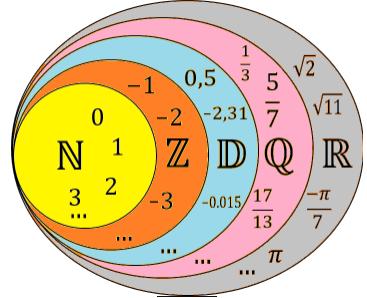
\includegraphics[width = 0.4\textwidth]{ensemble.PNG}
    \end{center}
\end{itemize}


\mysection{Opérations dans $\R$ et propriétés}

\mysubsection{1}{Règle fondamentales de développement et de factorisation}
\begin{Proposition}
    Soient $a,\ b$ et $c$ des nombres réels. On a :
    $$a\times(b+c) = a\times b + a\times c$$
    $$(b+c)\times a = b\times a + c\times a$$
    $$(a+b)(c+d) = ac + ad + bc +bd$$
\end{Proposition}

\begin{Exemple}
    \begin{enumerate}
        \item Dévellopement : $3(2x+5y)$ et $-\sqrt{2}(\sqrt{3}x - 4y)$ et $4x(x^2 + x - 3) $
        \item Factorisation : $13x + 26$ et $\sqrt{2}x + \sqrt{2}$ et $4(x-2) + (x-3)(x-2)$
    \end{enumerate}
\end{Exemple}

\newpage

\mysubsection{2}{Identités  remarquables}
\begin{Activité}
    Soient $a$ et $b$ deux nombres réels.
    \begin{enumerate}
        \item Développer $(a+b)^3$ et $(a-b)^3$
    \end{enumerate}
\end{Activité}
\begin{Proposition}
    Soient $a$ et $b$ deux nombres réels. On a :
    $$(a+b)^2 = a^2 + 2ab + b^2$$
    $$(a-b)^2 = a^2 - 2ab + b^2$$
    $$a^2 - b^2 = (a-b)(a+b)$$
    $$(a+b)^3 = a^3 + 3a^2b + 3ab^2 + b^3$$
    $$(a-b)^3 = a^3 - 3a^2b + 3ab^2 - b^3$$
    $$a^3-b^3 = (a-b)(a^2 + ab + b^2)$$
    $$a^3+b^3 = (a+b)(a^2 - ab + b^2)$$
\end{Proposition}

\begin{Exemple}
    \begin{enumerate}
        \item Développer : $(x + 3)^2\ ; \ (3a - 5)^2 \ ; \ (\sqrt{5} - \sqrt{3})(\sqrt{5} + \sqrt{3}) $
        \item Factoriser : $49x^2 - 25 \ ; \ x^2 + 2x - y^2 + 1 \ ; \ $
    \end{enumerate}
\end{Exemple}

\begin{Application}
    \begin{enumerate}
        \item Dévelloper : $A = (x + 2)^3 \ ; \ B = (2x - 3\sqrt{2})^3$
        \item Factoriser : $C = x^3 - 8 \ ; \ D = 8x^3 + 27$
        \item Calculer sans utiliser calculatrice : $99^2 \ ; \ 101^2$
    \end{enumerate}
\end{Application}

\mysection{Puissance d'un nombre}

\mysubsection{1}{Puissance d'un nombre réel}
\begin{Proposition}
     Soit $ a $ et $ b $ deux nombres réels non nuls et soit $ n $ et $ p $ deux entiers relatifs :
    \begin{multicols}{3}
        \begin{itemize}
            \item $ a^n \times a^p = a^{n+p} $
            \item $ (a^n)^p = a^{np} $
            \item $ \displaystyle\frac{1}{a^p} = a^{-p} $
            \item $ a^n \times b^n = (a \times b)^n $
            \item $ \displaystyle\frac{a^n}{a^p} = a^{n-p} $
            \item $ \displaystyle\frac{a^n}{b^n} = \displaystyle\left(\frac{a}{b}\right)^n $
        \end{itemize}
    \end{multicols}
\end{Proposition}

\begin{Exemple}
    \begin{multicols}{2}
        \begin{enumerate}
            \item $5^{-2}\times5^4 = 5^{-2+4} = 5^2$
            \item $\displaystyle\frac{3^4}{3^5} = 3^{4-5} = 3^{-1} = \displaystyle\frac{1}{3}$
            \item $(2^3)^2 = 8^2 = 64$
            \item $2^3\times 3^3 = (2\times 3)^3 = 6^3 = 216$
            \item $\displaystyle\frac{15^3}{5^3} = \displaystyle(\frac{15}{5})^3 = 3^3 = 27$
        \end{enumerate}
    \end{multicols}
\end{Exemple}

\newpage

\mysubsection{2}{Puissance du nombre 10}
\begin{Proposition}
    Pour tout entier naturel $n$, on a :
    \begin{center}
         $10^n =\underset{\underbrace{\hspace{1.5cm}}_{n \text{ zéros }}}{1000000000}$ \hspace{1.5cm} et \hspace{1.5cm} $10^{-n} =\underset{\underbrace{\hspace{1.5cm}}_{n \text{ zéros }}}{0.0000000001}$
    \end{center}
\end{Proposition}

\begin{Exemple}
    \begin{multicols}{2}
        \begin{enumerate}
            \item $10^5 = 100000$ (5 zéros)
            \item $10^{-4} = 0.00001$ (4 zéros)
            \item $10^{-7} = 0.00000001$ (7 zéros)
        \end{enumerate}
    \end{multicols}
\end{Exemple}
\mysubsection{3}{Écriture scientifique}
\begin{Définition}
    Tout nombre décimal positif peut s'écrire sous la forme $a\times 10^p$ où $a\in\D$ tel que $1\leq a\leq 10$ et $p\in\Z$.

    L'écriture $a\times 10^p$ s'appelle l'écriture scientifique.
\end{Définition}
\textcolor{red}{Remarque :}

Si le nombre est négatif, alors son écriture scientifique est : $-a\times 10^p$ où $a\in\D$ et $1\leq a\leq 10$ et $p\in\Z$.

\begin{Exemple}
    \begin{itemize}
        \item L'écritute scientifique du nombre $124,55$ est $1,2455\times 10^2$.
        \item L'écritute scientifique du nombre $0,00025$ est $2,5\times 10^{-4}$.
        \item L'écritute scientifique du nombre $11,00007$ est $1,100007\times 10^1$.
    \end{itemize}
\end{Exemple}

%
%&\\
%\hline
%\end{tabular}


\end{document}